\documentclass[UTF8,12pt]{article} % 12pt 为字号大小
\usepackage{amssymb,amsfonts,amsthm}
%\usepackage{fontspec,xltxtra,xunicode}
%\usepackage{times}
\usepackage{amsmath,bm}
\usepackage{mdwlist}
\usepackage[colorlinks,linkcolor=blue]{hyperref}
\usepackage{cleveref}

%----------
% 定义中文环境
%----------

\usepackage{xeCJK}
\usepackage{float}
\setCJKmainfont[BoldFont={Heiti SC Light},ItalicFont={Kaiti SC Regular}]{Songti SC Regular}
\setCJKsansfont{Heiti SC Light}
\setCJKfamilyfont{song}{Songti SC Regular}
\setCJKfamilyfont{zhhei}{Heiti SC Light}
\setCJKfamilyfont{zhkai}{Kaiti SC Regular}
\setCJKfamilyfont{zhfs}{STFangsong}
\setCJKfamilyfont{zhli}{Libian SC Regular}
\setCJKfamilyfont{zhyou}{Yuanti SC Regular}

\newcommand*{\songti}{\CJKfamily{zhsong}} % 宋体
\newcommand*{\heiti}{\CJKfamily{zhhei}}   % 黑体
\newcommand*{\kaiti}{\CJKfamily{zhkai}}  % 楷体
\newcommand*{\fangsong}{\CJKfamily{zhfs}} % 仿宋
\newcommand*{\lishu}{\CJKfamily{zhli}}    % 隶书
\newcommand*{\yuanti}{\CJKfamily{zhyou}} % 圆体

%----------
% 版面设置
%----------
%首段缩进
\usepackage{indentfirst}
\setlength{\parindent}{2em}

%行距
\renewcommand{\baselinestretch}{1.5} % 1.5倍行距

%页边距
\usepackage[a4paper]{geometry}
\geometry{verbose,
  tmargin=2cm,% 上边距
  bmargin=2cm,% 下边距
  lmargin=2.5cm,% 左边距
  rmargin=2.5cm % 右边距
}


%----------
% 其他宏包
%----------
%图形相关
\usepackage[x11names]{xcolor} % must before tikz, x11names defines RoyalBlue3
\usepackage{graphicx}
\graphicspath{{figures/}}
\usepackage{pstricks,pst-plot,pst-eps}
\usepackage{subfig}
\def\pgfsysdriver{pgfsys-dvipdfmx.def} % put before tikz
\usepackage{tikz}

%原文照排
\usepackage{verbatim}

%网址
\usepackage{url}

%----------
% 定理、习题与解答环境
%----------
%定理环境
\usepackage[most]{tcolorbox}
\newtcbtheorem[number within=section]{theorem}{定理}{
     enhanced,
     breakable,
     sharp corners,
     attach boxed title to top left={
       yshifttext=-1mm
     },
     colback=white,
     colframe=blue!75!black,
     fonttitle=\bfseries,
     boxed title style={
       sharp corners,
       size=small,
       colback=blue!75!black,
       colframe=blue!75!black,
     } 
}{theorem}

\newtcbtheorem[number within=section]{definition}{定义}{
     enhanced,
     breakable,
     sharp corners,
     attach boxed title to top left={
       yshifttext=-1mm
     },
     colback=white,
     colframe=blue!75!black,
     fonttitle=\bfseries,
     boxed title style={
       sharp corners,
       size=small,
       colback=blue!75!black,
       colframe=blue!75!black,
     } 
}{definition}

\newtcbtheorem[number within=section]{corollary}{推论}{
     enhanced,
     breakable,
     sharp corners,
     attach boxed title to top left={
       yshifttext=-1mm
     },
     colback=white,
     colframe=blue!75!black,
     fonttitle=\bfseries,
     boxed title style={
       sharp corners,
       size=small,
       colback=blue!75!black,
       colframe=blue!75!black,
     } 
}{corollary}

\newtcbtheorem[number within=section]{myboxes}{盒子}{
     enhanced,
     breakable,
     sharp corners,
     attach boxed title to top left={
       yshifttext=-1mm
     },
     %colback=white,
     colframe=black!75!white,
     fonttitle=\bfseries,
     boxed title style={
       sharp corners,
       size=small,
       colback=black!75!white,
       colframe=black!75!white,
     } 
}{myboxes}

%习题环境
\newtcbtheorem[]{exercise}{题}{
     enhanced,
     breakable,
     sharp corners,
     attach boxed title to top left={
       yshifttext=-1mm
     },
     colback=white,
     colframe=black,
     fonttitle=\bfseries,
     boxed title style={
       sharp corners,
       size=small,
       colback=black,
       colframe=black,
     } 
}{Problem}

%解答环境
\ifx\proof\undefined\
\newenvironment{proof}[1][\protect\proofname]{\par
\normalfont\topsep6\p@\@plus6\p@\relax
\trivlist
\itemindent\parindent
\item[\hskip\labelsep
\scshape
#1]\ignorespaces
}{%
\endtrivlist\@endpefalse
}
\fi

\renewcommand{\proofname}{\it{Solution}}

%----------
%示例:
%\begin{exs} \end{exs}
%\begin{proof}[] \end{proof}
%\begin{thm}{}{} \end{thm}
%----------

%----------
%插入图片
%\begin{figure}[htbp]
%\centering
%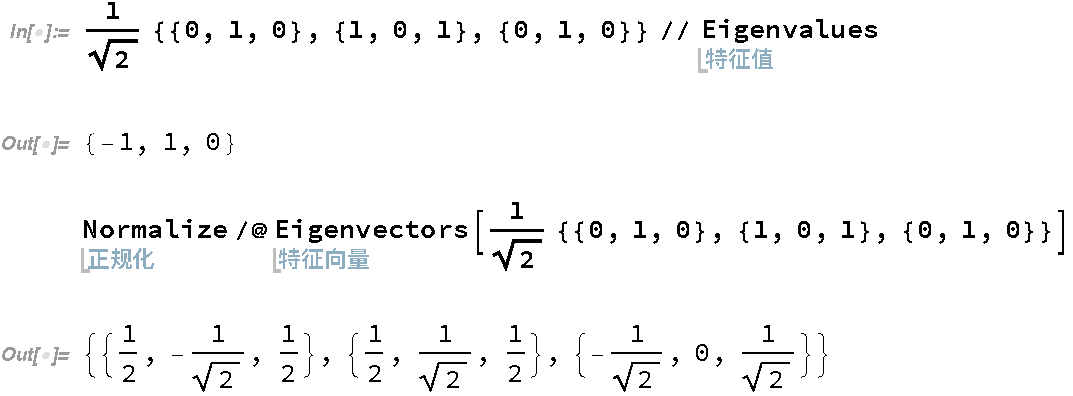
\includegraphics[width=10cm]{eigen}
%\end{figure}
%----------

%==========
% 正文部分
%==========

\begin{document}

\title{作业 07}
\author{陈昱全~SA18234049}
\date{} % 若不需要自动插入日期,则去掉前面的注释;{ } 中也可以自定义日期格式
\maketitle

\begin{exercise}{}{}
With $$\sigma_x = \begin{pmatrix}0&1\\1&0\end{pmatrix},~ \sigma_y = \begin{pmatrix}0&-i\\i&0\end{pmatrix},~ \sigma_z = \begin{pmatrix}1&0\\0&-1\end{pmatrix}$$ and $$\vec{n} = (sin\theta cos\varphi, sin\theta sin\varphi, cos\theta),~ \vec{\sigma} = (\sigma_x, \sigma_y, \sigma_z)$$ find eigenvalue and eigenstates of $\vec{\sigma}\cdot\vec{n}$
\end{exercise}

\begin{proof}[解]
直接用Mathematica求解如下
\begin{figure}[H]
\begin{center}
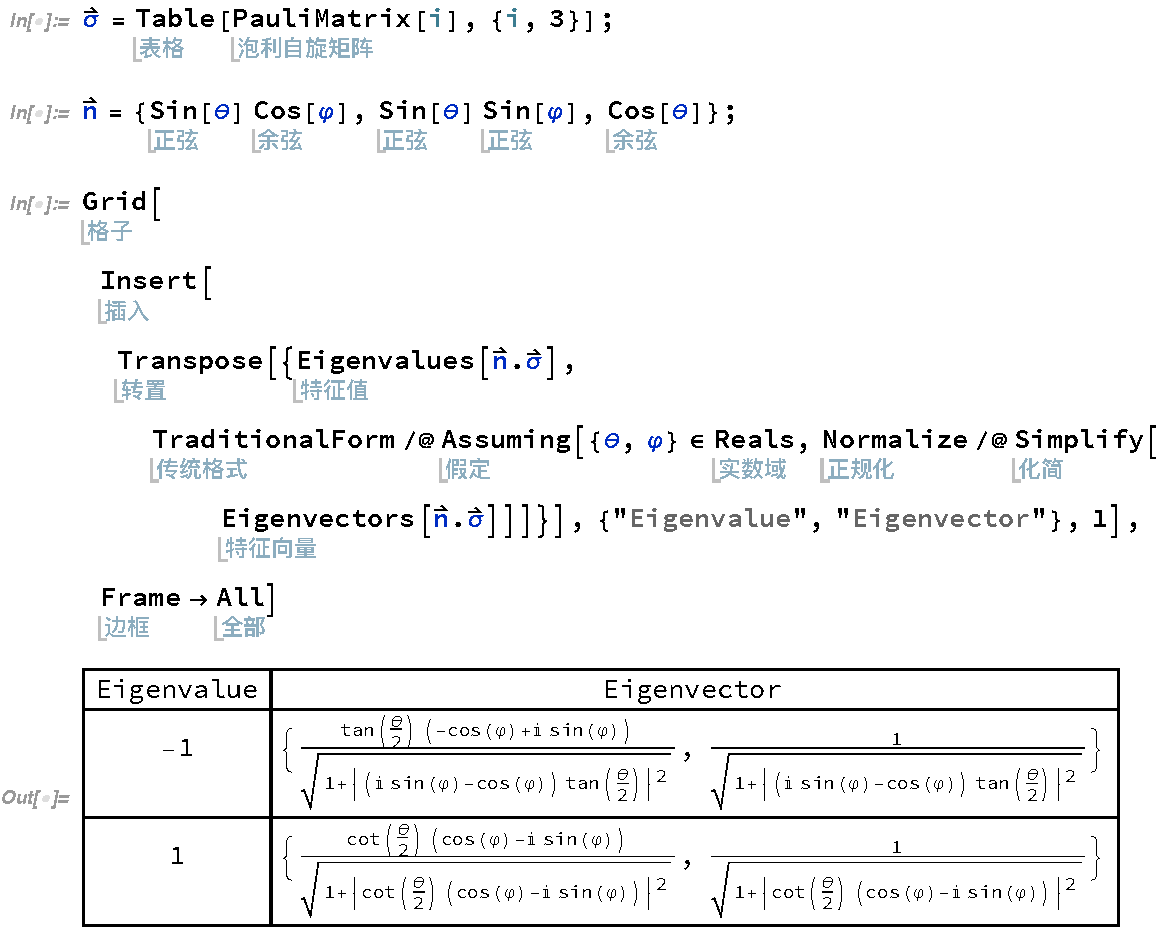
\includegraphics[width=15cm]{prob1}
%\caption{}
%\label{}
\end{center}
\end{figure}
\end{proof}

\begin{exercise}{}{}
With $\psi(\theta,\varphi) = \frac{1}{\sqrt{3}}\left(\sqrt{2}Y_1^0(\theta,\varphi) + Y_1^1(\theta,\varphi)\right)$, without integrations, find $\langle L^2\rangle, \langle L_z\rangle$
\end{exercise}

\begin{proof}[解]
我们已知
\begin{align*}
L_z Y_{lm} &= m\hbar Y_{lm} \\
L^2 Y_{lm} &= l(l+1)\hbar^2 Y_{lm}
\end{align*}
所以
\begin{align}
L^2|\psi\rangle &= L^2\left(\sqrt{\frac{2}{3}}Y_1^0 + \sqrt{\frac{1}{3}}Y_1^1\right) = \sqrt{\frac{2}{3}}2\hbar^2Y_1^0 + \sqrt{\frac{1}{3}}2\hbar^2Y_1^1 \\
L_z|\psi\rangle &= \sqrt{\frac{1}{3}}\hbar Y_1^1
\end{align}
故
\begin{align}
\langle L^2\rangle &= 2\hbar^2 \\
\langle L_z\rangle &= \frac{\hbar}{3}
\end{align}
\end{proof}

\begin{exercise}{}{}
With $\phi(t=0) = \psi(\theta,\varphi)$ as above, $H = \frac{\vec{L}^2}{2mR^2}$, find $\phi(t=T)$
\end{exercise}

\begin{proof}[解]
因为
\begin{align}
L^2 |l,m\rangle = l(l+1)\hbar^2 |l,m\rangle
\end{align}
我们可以把算符$L^2$展开为
\begin{align}
L^2 = \sum l(l+1)|l,m\rangle\langle l,m|
\end{align}
同样可以把演化算符$e^{-\frac{i}{\hbar}Ht}$做如下展开:
\begin{align}
e^{-\frac{i}{\hbar}Ht} &= e^{-\frac{it}{2m\hbar R^2}L^2} \notag\\
&= \sum e^{-\frac{it}{2m\hbar R^2}l(l+1)} |l,m\rangle\langle l,m|
\end{align}
所以
\begin{align}
\phi(t) &= e^{-\frac{i}{\hbar}Ht}\phi(0) \notag\\
&= \left(\sum e^{-\frac{it}{2m\hbar R^2}l(l+1)} |l,m\rangle\langle l,m|\right) \left(\sqrt{\frac{2}{3}}|1,0\rangle + \sqrt{\frac{1}{3}}|1,1\rangle\right) \notag\\
&= e^{-\frac{it}{mR^2\hbar}}\left(\sqrt{\frac{2}{3}}Y_1^0 + \sqrt{\frac{1}{3}}Y_1^1\right)
\end{align}
\end{proof}

\begin{exercise}{Uncertainty principle}{}
With $J_z|j,m\rangle = m\hbar|j,m\rangle, \vec{J}^2|j,m\rangle = \hbar^2 j(j+1)|j,m\rangle$, $$\langle\Delta A\rangle = \sqrt{\langle j,m|A^2|j,m\rangle - (\langle j,m|A|j,m\rangle)^2}$$ find $\langle\Delta J_x\rangle\langle\Delta J_y\rangle$ and $\langle[J_x, J_y]\rangle$, check $\langle\Delta J_x\rangle\langle\Delta J_y\rangle\ge\frac{1}{2}|\langle[J_x, J_y]\rangle|$.\\ When $\langle\Delta J_x\rangle\langle\Delta J_y\rangle = \frac{1}{2}|\langle[J_x, J_y]\rangle|$, what's the requirement of $m$?
\end{exercise}

\begin{proof}[解]
我们先证明在$J_z$的本征态$|j,m\rangle$下,$\langle J_x\rangle = \langle J_y\rangle = 0$。因为
\begin{align}
[J_y, J_z] = i\hbar J_x
\end{align}
两边在$|j,m\rangle$态下求平均值,
\begin{align}
\text{LHS} &= \langle j,m|J_yJ_z - J_zJ_y|j,m\rangle = m\hbar\langle j,m|J_y|j,m\rangle - m\hbar\langle j,m|J_y|j,m\rangle = 0 \\
\text{RHS} &= i\hbar\langle j,m|J_x|j,m\rangle = i\hbar\langle J_x\rangle
\end{align}
故有$\langle J_x\rangle = 0$,同理可得$\langle J_y\rangle = 0$。由对称性,可知$\langle\Delta J_x\rangle = \langle\Delta J_y\rangle$,又有
\begin{align}
\langle\Delta J_x\rangle^2 = \langle J_x^2\rangle - \langle J_x\rangle^2 = \langle J_x^2\rangle
\end{align}
则
\begin{align}
\langle\Delta J_x\rangle^2 &= \langle\Delta J_y\rangle^2 = \frac{1}{2}\left(\langle\Delta J_x\rangle^2 + \langle\Delta J_y\rangle^2\right) \notag\\
&= \frac{1}{2} \left(\langle J_x^2\rangle + \langle J_y^2\rangle\right) = \frac{1}{2} \langle J_x^2 + J_y^2\rangle \notag\\
&= \frac{1}{2} \langle J^2 - J_z^2\rangle = \frac{1}{2} (\langle J^2\rangle - \langle J_z^2\rangle) \notag\\
&= \frac{1}{2} \left[j(j+1) - m^2\right]\hbar^2
\end{align}
我们已知$[J_x,J_y]=i\hbar J_z$,则$\left|\langle[J_x,J_y]\rangle\right| = \left|i\hbar\langle J_z\rangle\right| = \left|m\right|\hbar^2$,
\begin{align}
\langle\Delta J_x\rangle\langle\Delta J_y\rangle &= \langle\Delta J_x\rangle^2 = \frac{1}{2} \left[j(j+1) - m^2\right]\hbar^2 \\
&\ge \frac{1}{2} \left|m\right|\hbar^2
\end{align}
当$m = \pm j$时取等号。
\end{proof}

\begin{exercise}{}{}
Write out $J_- J_+$ as a matrix in the basis of $J_z$, with $j=1$, and find the eigenvalue and eigenstates of $J_-J_+$
\end{exercise}

\begin{proof}[解]
\begin{align}
J_-J_+ &= \left(J_x + iJ_y\right)\left(J_x - iJ_y\right) \\
&= J_x^2 -i[J_x, J_y] + J_y^2 \notag\\
&= J_x^2 + \hbar J_z + J_y^2 \notag\\
&= J^2 - J_z^2 + \hbar J_z
\end{align}
\end{proof}



\end{document}